\chapter{Inventing Color}\footnote{Contributions from Brent Barker, Mike Gladders, Amanda Pagul, and others.}

%todo for in-person lab: subtraction of colors for filter part does not work. magnitudes are already logarithmic, so it works for them. Try doing measurements and using ratio of g/r instead of difference, adjust lab accordingly.

%TODO rewrite rgb image directions. these are very unclear.

%TODO for "conduct an experiment", be more clear about what deliverables / product is wanted

Everything glows (gives off electromagnetic radiation) when it has a temperature --- particles are wiggling around randomly (faster if it's hotter) and giving off energy as they wiggle. This \textbf{thermal radiation}, also called blackbody radiation, is the same for any object at the same temperature. The spectral density $B$ of this radiation at wavelength $\lambda$ and temperature $T$ is given by Planck's Law:
\begin{equation}\label{ic:eq:planck}
 B(\lambda, T) = \frac{2 h c^2}{\lambda^5}
 \frac{1}{\exp\left( \frac{hc}{\lambda k_\textrm{B} T} \right) - 1} \,,
\end{equation}
where $h$ is the Planck constant, $c$ is the speed of light in the medium, and $k_\textrm{B}$ is the Boltzmann constant. The peak of this distribution $\lambda_\textrm{peak}$ is given by Wien's displacement law,
\begin{equation}\label{ic:eq:wien}
	\lambda_\textrm{peak} = \frac{b}{T} \,,
\end{equation}
where $b \approx 2898\:\mu$m$\cdot$K is Wien's displacement constant. This universal behavior means we can take something's temperature by looking at the spectrum of light it gives off. This is great for learning about something's temperature at a distance, like stars.

%Incandescent lightbulbs are so warm that they glow in the visible spectrum (like stars). In this lab, you'll investigate the radiation that is given off by a lightbulb at various temperatures, then use filters to mimic the situation astronomers are in when they observe astronomical objects with different color filters. You'll invent a metric to numerically state the temperature of the lightbulb, even without knowing the actual temperature. Finally, you'll use the various images that you took with SEO with different color filters and combine them to form a color image.

\section{Forming Groups}

If you are attending the lab session live and do not yet have a group, one way the TA could assist is to arrange "speed networking" among those who still need a group. This would involve the TA organizing Zoom Breakout Rooms, where each room is 2-3 students, and each group talks about how they work and what they are looking for in a group member. Then after 5 minutes or so, the Rooms are changed so people are with different people. This could help people get to know each other enough to form lab groups.

\begin{steps}
	\item\label{ic:step:team-comm} Once you have a group, meet with each other and decide a) what tools you will use to communicate and collaborate, b) when you will meet, c) what you will do when you need to change an agreement, and d) what you will do when you a person has an issue with how the group is functioning.
	\textbf{Write this in your lab report. This part counts as data collection and analysis, so it can be identical in each member's report.}
\end{steps}

\section{Team roles}

\textbf{Decide on roles} for each group member. The available roles are:

\begin{itemize}
	\item Facilitator: ensures time and group focus are efficiently used
	\item Scribe: ensures work is recorded
	\item Technician: oversees apparatus assembly, usage
	\item Skeptic: ensures group is questioning itself
\end{itemize}

These roles can rotate each lab, and you will report at the end of the lab report on how it went for each role. If you have fewer than 4 people in your group, then some members will be holding more than one role. For example, you could have the skeptic double with another role. Consider taking on a role you are less comfortable with, to gain experience and more comfort in that role.

Additionally, if you are finding the lab roles more restrictive than helpful, you can decide to co-hold some or all roles, or think of them more like functions that every team needs to carry out, and then reflecting on how the team executed each function.

\section{Exploring thermal radiation}\label{ic:sec:exploring}

\begin{steps}
	\item\label{ic:step:load-sim} Load the interactive thermal radiation simulation at \url{https://phet.colorado.edu/sims/html/blackbody-spectrum/latest/blackbody-spectrum_en.html}
	
	\item Play with the controls and see what happens. Discuss among your team.
	
	\item Find a pattern --- how does the shape change as the temperature goes up? For example, how does the peak wavelength change, and how about the total radiated power (area under curve)? \textbf{Record your observations.}
	
	\item At what peak wavelength do you radiate? Use the sim to determine this and estimate your uncertainty. \textbf{Record your findings.}
	
	\item Using your estimated temperature, calculate your peak wavelength according to Wien's law.
	
	\item\label{ic:step:qual-color} Comparing the spectra of the light bulb, Sun, and Sirius A, how can you use the spectrum to determine what color each one appears as?
\end{steps}

\section{CCDs and filters}

Cameras have come a long way since the days of developing film, but sensors are not as smart you might think. They register light, but they can't usually tell the color (i.e. wavelength) of the incoming photons. So then how do you get a color image? In astronomy (and in your cell phone!) color images are generated by measuring the amount of light at specific colors and then combining these measurements to create a colorful image. A filter is used to select bands of color to allow through. In consumer cameras and phone cameras, these filters are permanently attached to the front of individual pixels. In astronomical imaging, there is no permanent filter, and different filters are moved into place.

\subsection{Filters}
Light is composed of photons with energies that determine their wavelengths (shorter wavelength $\implies$ higher energy). Thus every light source exhibits a \textbf{spectrum} of energies based on its energetic components, determined by the physics of the light emission process. Thus, observing the energetic constituents of light from astronomical objects - a.k.a. observing the spectrum of emitted radiation - is a fundamental tool in observational astrophysics. However, obtaining the specific intensity of radiation as a function of energy from an astronomical source is challenging. An easier way to asses the electromagnetic energies observed is to image them in different filters: materials that are transparent to a known range of wavelengths and opaque to all others. Thus, one can image the same object with multiple different filters to get a sense of the wavelength regimes that make the strongest contributions to the overall electromagnetic output.

A filter is characterized by its \textbf{transmission function}: a function that characterizes the amount of light that is transmitted by the filter at each wavelength. Figure~\ref{sot:fig:filters} shows the transmission functions for standard astronomical filters that are used in the Sloan Digital Sky Survey and now used as standard filters elsewhere.% (similar to the ones you'll be using in this class).

\begin{figure}
	\centering
	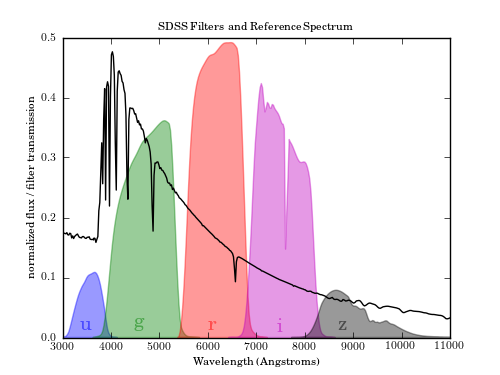
\includegraphics{small-optical-telescopes/fig_sdss_filters_1.png}
	\caption{Filter Transmission Functions for the Sloan Digital Sky Survey, overlaid on a stellar spectrum (in this case the spectrum is probably an
		A-type star). The magnitude observed by each filter will be proportional to the integrated spectrum multiplied by the filter transmission. It's clear in this image that the underlying spectrum of the star will cause the different filters to have different magnitudes. How would these magnitudes change if the spectrum was, say, of an M-star instead? (Image source: \url{http://www.astroml.org/\_images/fig\_sdss\_filters\_1.png})}\label{sot:fig:filters}
\end{figure}

\begin{steps}
	\item Open the Google Sheet found here: \url{https://docs.google.com/spreadsheets/d/1qgTqiqWOFCzYuSmHeT-5hwy_lBYO0Tvu24kM955nfq4/edit?usp=sharing}
	
	\item Make a copy of this sheet for your group to use.
\end{steps}

This spreadsheet calculates the same theoretical thermal radiation curve (according to Planck's Law) as the PhET simulation above, seen in the first two columns. Then it applies the transmission functions of the SDSS filters and plots the remaining power spectrum that gets through each filter. Finally, it sums up each filter's power spectrum and gives a total pixel value and magnitude. The pixel value is the relative number of counts a pixel with that filter would read. This is proportional to the brightness it sees.

\subsection{Magnitude}

Astronomers measure brightness of stars using a measurement system called \textit{magnitude}. About two millenia ago, astronomers categorized stars into 6 different brightness classes, 1st class through 6th class. When brightness began to be more quantified, it was found that first magnitude stars were about 100 times brighter than 6th magnitude stars. Then it was decided to scale the 6 classes logarithmically, to account for the several orders of magnitude involved. The relationship between intensity (power per unit area) \textit{I} and magnitude $m$ is defined as
\begin{equation}
 m \equiv -2.5 \log_{10} \left(\frac{I}{I_\textrm{ref}}\right) \,,
\end{equation}
where $I_\textrm{ref}$ is the intensity of some standard reference object. In the spreadsheet, these values marked as magnitudes are not technically magnitudes, since we are not using the dimensions of intensity, but it will help your analysis to treat them as such.

\subsection{Color index}

In Section \ref{ic:sec:exploring}, you learned that the color of a thermally radiating object is related to its temperature. Here, you will develop a quantitative color index and use it to determine the temperature of the Sun.

\begin{steps}
	\item\label{ic:step:see-thermal} In the spreadsheet, change the temperature of the blackbody (edit cell \texttt{B1}) and watch how the spectrum changes, and how the filter magnitudes change with respect to each other. \textbf{Record your observations.}
\end{steps}
	
The magnitude depends not just on the temperature, but also on the size of the star and the distance away from us. So to characterize a star's color quantitatively, independent of the size and distance, astronomers use a ratio of brightnesses of different filters. This is equivalent to subtracting the magnitudes. The subtraction of two broadband filter magnitudes is called the \textit{color index}.

\subsection{Correlating color index and temperature}

In order to use the color index of a star to find its temperature, you need to determine how the two related to each other. If you assume the EM radiation emitted by the star is entirely due to thermal radiation, then you can find the theoretical color index of a blackbody at various temperatures, and then find where the star's color index sits on that graph.

\begin{steps}
	\item Choose the filters from which to make your color index. Do you want to choose filters that detect wavelengths right next to each other, or farther apart? If you're not sure, try both and see which is better for this application. You can call the resulting color index ``$x - y$'', for example $g' - r'$ if you are subtracting the $r'$ filter value from the $g'$ value.
	
	\item\label{ic:step:tempcolor} Make a table and graph of temperature vs. color index. \textbf{Record your table and graph.}
\end{steps}

\subsection{Taking the Sun's temperature}

\begin{steps}
	\item Switch to the ``Sun'' tab in the spreadsheet. This has experimentally determined values for the intensity of EM radiation impinging on the Earth from the Sun, alongside the same filtering system as in the theoretical tab.
	
	\item\label{ic:step:proc-color} Design a procedure to use the filter magnitudes of the Sun to determine its temperature and your uncertainty of that temperature. Run this procedure by your TA to get feedback on it before starting.
	
	\item Conduct your experiment and keep a log.
	
	\item Look up the effective temperature of the Sun's photosphere on Wikipedia.
	
	\item Calculate the percent difference between your value and the one that Wikipedia references:
	\begin{equation}
	 \textrm{percent difference} = \frac{\abs{a-b}}{\frac{a+b}{2}} \times 100\%
	\end{equation}
	
	\item\label{ic:step:solar-compare} Use the $t'$ statistic described in Appendix\ \ref{unc:sec:comparing} to compare the two values and interpret the result --- do these two measurements really measure the same thing? If they are very different, check your procedure, and if the difference stays, discuss what could be different about the methods used to find the temperature, or different assumptions used. \textbf{Record your discussion.}
\end{steps}

%\section{Lightbulbs}
%
%Light can be made of many different wavelengths at the same time. It combines to form a color that we perceive. To see what colors make up light, we can split them again with a triangular prism, or with a \textit{diffraction grating}.
%
%\begin{steps}
%	\item Use the diffraction grating to view the lightbulb while the lightbulb is at full voltage (120 V). Hold up the grating in front of your eye, with the text on the frame upright. Start by looking at the lightbulb through it, then turn your feet to the left or right about 30 degrees, letting your whole body-arm-grating system rotate with your feet. You should see a rainbow. This is all the colors that make up the light coming from the lightbulb, split into different wavelengths.
%\end{steps}
%
%\subsection{Orientation to the digital spectrometer}
%
%\begin{framed}
%	\textbf{Warning! Fragile Equipment!} If the fiber optic cable is bent into a circle of less than 9 cm (6 inch) diameter, then the fiber inside may break.
%	
%	Also, the blue end cap should be replaced on the end of the fiber optic cable when you are done using it, to protect from dust and debris entering.
%\end{framed}
%
%A digital spectrometer also uses a diffraction grating, but instead of collecting the dispersed light on a screen to be viewed by people, it collects the light with a charge-coupled device (CCD), an array of light-sensitive pixels much like a digital camera. It then translates the position on the CCD to individual wavelengths and displays a plot of intensity vs. wavelength on a computer. %TODO (see Figure~???)
%Another difference is that we use an optical fiber to collect the light.
%
%Here are a few guidelines:
%\begin{itemize}
%	
%	\item \textbf{Background subtraction.} When you are observing the spectrum of something, there may be stray light entering that is not coming from the thing you are studying. To remove this \textit{background} from the plot, select the gray lightbulb icon in the toolbar. This records the current plot as the background. To display the plot while subtracting the background, select the icon with the minus-lightbulb. To go back to viewing the full spectrum including the background, select the blue S icon.
%
%	\item \textbf{Oversaturation}. If, when you zoom out all the way, the plot includes a flat line near the top of the plot, this means that the pixels of the image sensor are recording their maximum value, and they cannot tell you the actual intensity. Reduce the intensity by either reducing the integration time (upper-left corner) or moving the fiber optic cable off-center, so that it receives less light. Note that if you change either of these, then the background frame is no longer correct and must be remeasured.
%
%	\item \textbf{Low signal}. If the target is dim, then you might find when you zoom in, the plot is not smooth, but instead jagged and hard to find patterns in. In this case, increase the integration time using the field in the upper-left of the program window. This increases the exposure time, equivalently. Note that if you change the integration time, then the background frame is no longer correct and must be remeasured.
%
%	\item \textbf{Saving data.}
%	
%	\begin{itemize}
%		\item Save the images of spectra and numeric files that you generated with SpectraSuite
%	during your experiments on a USB stick, so that you can use them at home during
%	preparation of your report (you can also email them as attachments from your
%	computer at the end of the lab).
%	
%	\item You should open a word processor document and a spreadsheet document in which you can save your measured
%	spectra at the beginning of your work. To save an image of your graph, click on
%	the fourth icon from the left in the Spectrum IO controls. %TODO (Fig.~???)
%	This will copy
%	an image of the graph to the clipboard. Then in your word processor, paste the image by pressing
%	Ctrl-V.
%	
%	\item To save spectrum in the digital form, click on the third from the left icon in
%	Spectrum IO controls (to the right of print icon). This copies it to clipboard. In
%	Excel file make sure you are in a new sheet and press Ctrl-V. This should create
%	to columns of numbers: wavelength (in nm) and counts for your spectrum.
%	
%	\item An alternative way to save the data is to click on the floppy disk icon in the
%	Spectrum IO controls. The format must be ``Tab delimiter, no header''. The
%	writing directory must be specified (``Browse'' button). The spectrum is saved in a
%	text file (.txt) as two columns, the first column giving the wavelength in nm, the
%	second column the corresponding intensity. This file can be imported into a spreadsheet or plotting program.
%	\end{itemize}
%\end{itemize}
%
%\subsection{Observing a lightbulb}
%
%\begin{steps}
%	
%	\item Using the spectrometer, observe the spectrum created by a lightbulb at various brightnesses / voltages.  What's the overall shape? \textbf{Record your answer.}
%	
%	\item How does the shape change when the brightness increases? \textbf{Record your answer.}
%	
%	\item How does the peak frequency change? \textbf{Record your answer.}
%	
%	\item How does the visual color of the bulb change as it gets brighter? \textbf{Record your answer.}
%	
%	\item\label{ic:step:pattern} As the lightbulb gets brighter, the filament inside gets hotter --- the temperature increases. If all objects act like the tungsten filament as it gets hotter, what general pattern can you state about the light given off by an object as a function of its temperature? \textbf{Record your answer.}
%
%\end{steps}
%
%Cameras have come a long way since the days of developing film, but sensors are not as smart you might think. They register light, but they can't usually tell the color (i.e. wavelength) of the incoming photons. So then how do you get a color image? In astronomy (and in your cell phone!) color images are generated by measuring the amount of light at specific colors and then combining these measurements to create a colorful image. A filter is used to select bands of color to allow through. In consumer cameras and phone cameras, these filters are permanently attached to the front of individual pixels. In astronomical imaging, there is no permanent filter, and different filters are moved into place.
%
%\begin{steps}
%	\item View the lightbulb's spectrum with the diffraction grating again, this time alternately holding the red and green filters between the grating and the bulb. Observe and \textbf{record} the effect of the filter on the spectrum.
%	
%	\item Use the red and green filters in front of the fiber optic input to the spectrometer to see how they affect the spectrum that is received. \textbf{Save a graph of the spectrum with each filter and include in your report.}
%\end{steps}
%
%In a regular astronomical image, each pixel gives just one value --- the number of counts detected in that pixel, regardless of the wavelength of the photon detected. We can treat the fiber optic as a single-pixel camera if we count up the total number of counts detected. To find that total number, you can find the area under the curve in the plot.
%
%\begin{steps}
%	\item With no filter, add up the total number of counts detected by calculating the area under the curve. To do this in an approximate way, count the number of boxes underneath the curve, then multiply this by the height of one box (in counts per nanometer) and by the width of one box (in nanometers). \textbf{Record this value.}
%	
%	\item Do the same for the spectrum using the red and green filters separately. Note that the values are different for different filters. This difference (for example, the green value minus the red value) can tell us a quantitative number for what color this object is. \textbf{Record the red, green, and $g-r$ values.}
%\end{steps}
%
%Now you have the value of our single-pixel camera for the case of clear (no filter), red, and green filters. Time to revisit the pattern found above in Step \ref{ic:step:pattern}.
%
%\begin{steps}
%	\item If that pattern from Step \ref{ic:step:pattern} is true, what should happen to the relative values of red and green as the voltage is increased? Should one increase more than the other? What should happen to the quantitative color $g-r$? \textbf{Record your answers.}
%	
%	\item Perform an experiment to test whether this prediction is supported. \textbf{Record your procedure, analysis, and results.}
%\end{steps}

\section{Creating a color image}

To create the beautiful color astronomy images we like to see, one must manually combine images taken with different filters. There are always choices to be made that will change how the combined image looks.

\begin{steps}
	\item\label{ic:step:color-image} Using the directions below, create a false color image of either the Orion nebula (M42), a stellar nursery, or the Crab nebula (M1), the remnant of a supernova. You can find the relevant images on Canvas in the Lab module.
\end{steps}

Now you'll create a color image from three separate images of the same target. You can use the broadband filters that you used in the previous section, and you can also try using the narrowband filters h-alpha, oiii, and sii. These filters only allow specific wavelengths through, that correspond to particular electronic excitations of hydrogen, oxygen, and silicon, respectively. Different features can be seen with different filters, as seen in Figure \ref{ic:fig:m1-filters}.

\begin{figure}
	\centering
	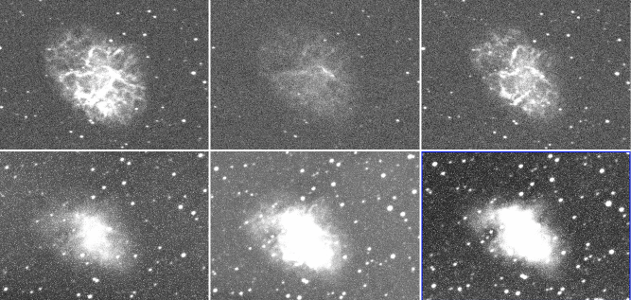
\includegraphics[width=\textwidth]{inventing-color/m1-different-filters-lores.png}
	\caption{Images of M1, the Crab Nebula, in different wavelength filters, revealing different features. Top row from left to right are the narrowband h-alpha, oiii, and sii filters. Bottom row is the broadband g', r', and i'. The structure comes out nicely in the narrowband, while there are more stars in broadband.}\label{ic:fig:m1-filters}
\end{figure}

Since there is not a 1-to-1 correspondence between the red-green-blue options in DS9 and the filters available, you will assign a different, arbitrary filter to each color in DS9. This makes the image a \textit{false color image}, since the colors we will see in it do not correspond to the actual wavelength of the light captured.

\textbf{Loading and manipulating images in ds9 consists of:}
\begin{itemize}
\item loading an image  (file $>$ open)
\item setting lower, upper limits (z1,z2) on an image  (scale $>$ various algorithms; use scale $>$ scale parameters for full control). See Figures \ref{ic:fig:z-min-max}--\ref{ic:fig:z-small} for examples.
\item controlling the intensity mapping within those bounds (mouse right click-and-hold and drag)
\end{itemize}

\begin{figure}
	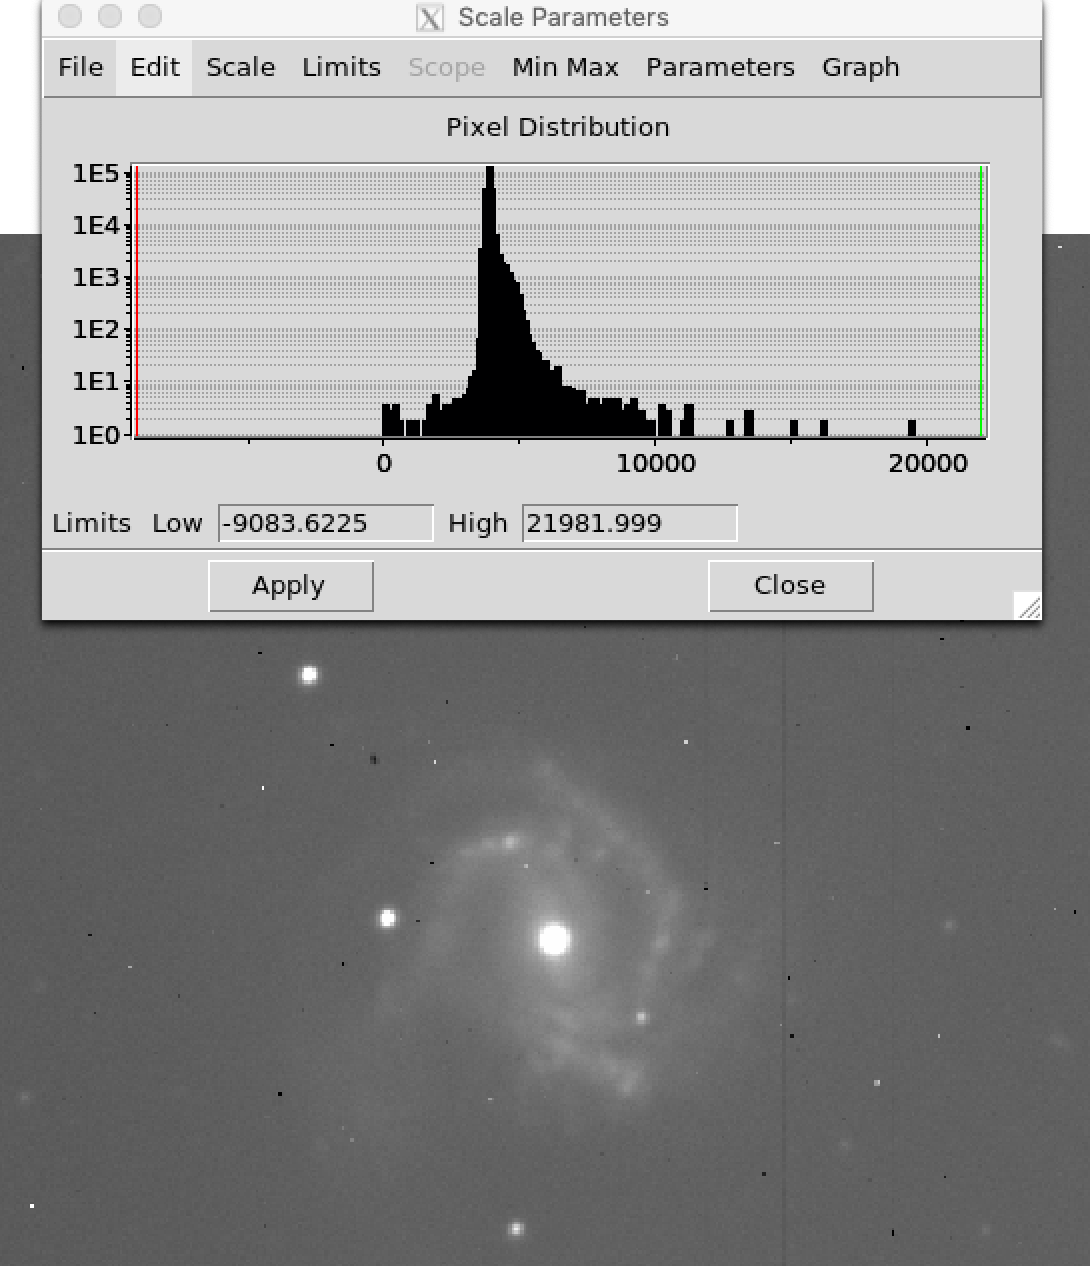
\includegraphics[width=0.5\textwidth]{inventing-color/z-min-max}
	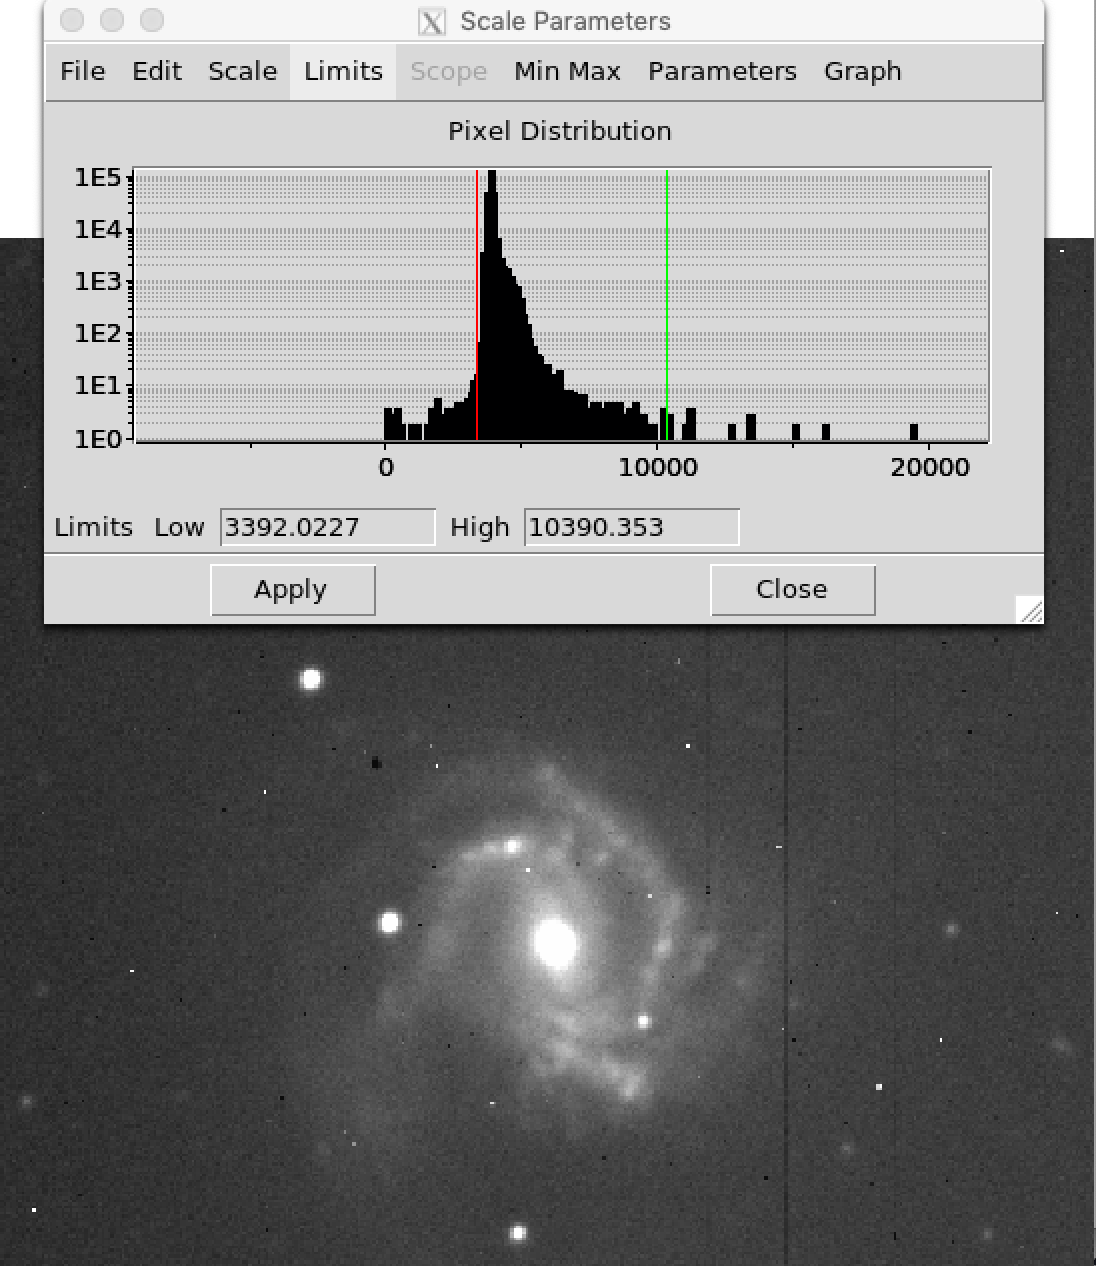
\includegraphics[width=0.5\textwidth]{inventing-color/z-mid}
	\caption{Proper choice of data ranges is important. The default for ds9 is often the min/max values in the image, which can be a poor choice if there are outlier pixels, as shown here on the left. The red line shows the lower limit z1, which is mapped to no color (black here), and the green line is the upper limit z2, mapped to full color (white here). Pixel values between these are shown in various brightnesses of the color. On the right, z1 and z2 are more tuned to the distribution of pixel values, which more effectively uses the dynamic range of the display for pixel values where there are significant amounts of data.}\label{ic:fig:z-min-max}
\end{figure}

\begin{figure}
		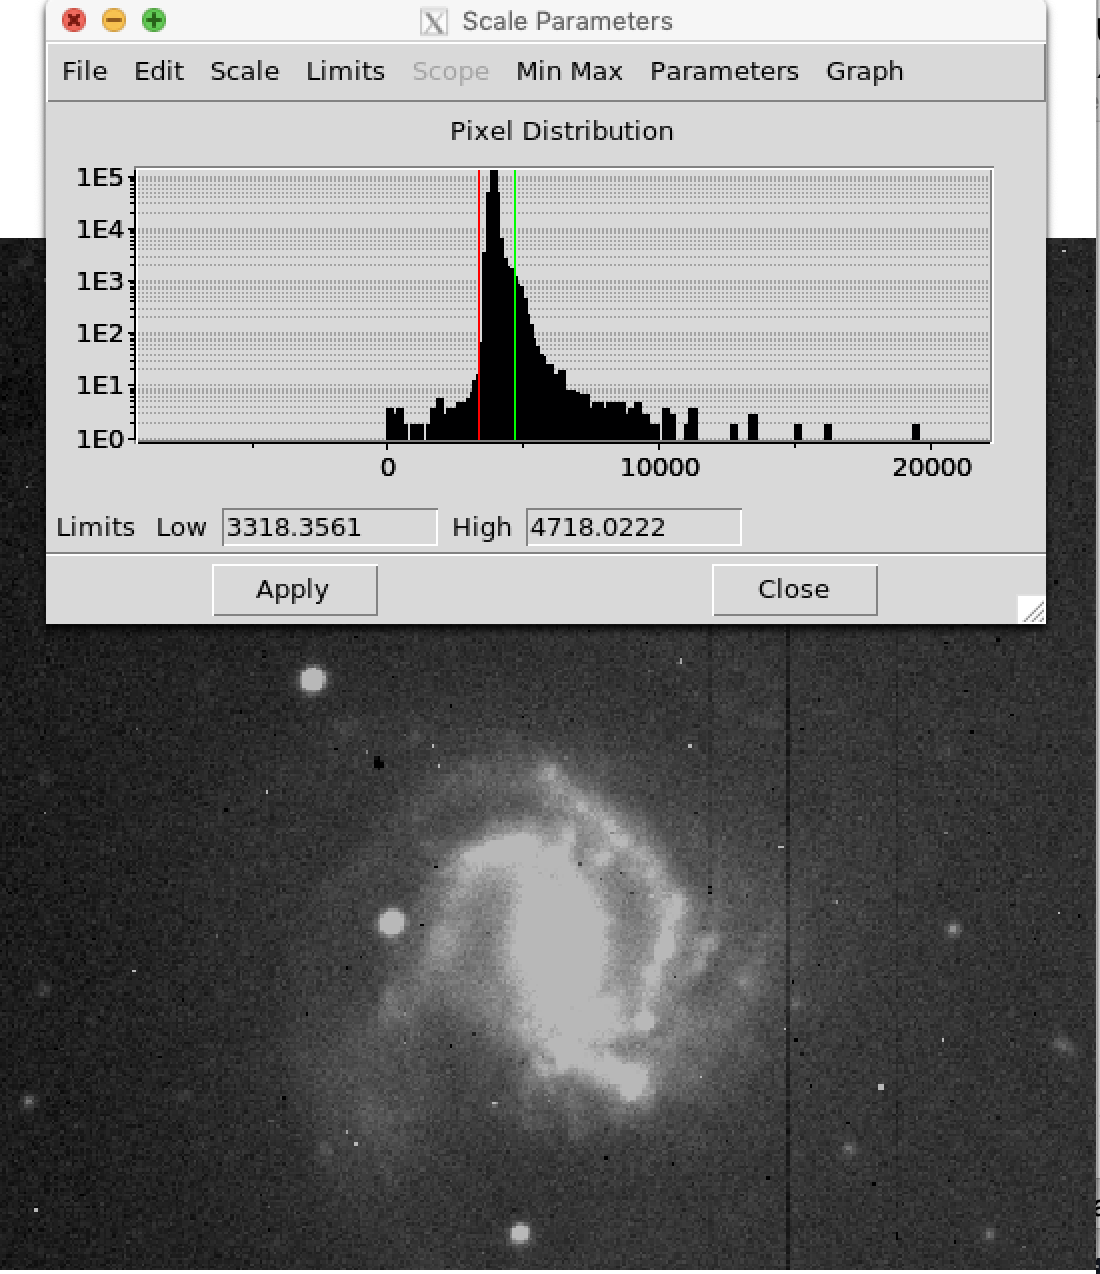
\includegraphics[width=0.5\textwidth]{inventing-color/z-small}
		\caption{Smaller values of z2 will emphasize fainter values in the target. Compare the image to the left to the right-hand image above.}\label{ic:fig:z-small}
\end{figure}

\textbf{You can change the zoom and center location in an image by} 
\begin{itemize}
\item moving around in image (mouse middle click if edit$>$point is set[the default], or edit$>$pan and mouse left click)
\item zooming in and out (mouse wheel, zoom$>$ +,- etc.)
\end{itemize}

\textbf{To build a color image}
\begin{itemize}
	\item Identify and download from SEO your three different filter image FITS files.
\item Open a color (rather than monochrome) frame:  Frame $>$ new rgb
\item Open the red, green, infrared files using the rgb subwindow to select which channel you are working in, and then scale and control intensities on each one. 
\item There are many possible ways to scale the images. Some testing suggests that choosing Scale $>$ ASINH (or Linear or Square Root as other choices) and Scale $>$ 99.5\% (or maybe 99\% or 98\%)  produces reasonable results. Experiment!
\item One thing to note: the rgb subwindow allows you to control how the images are aligned spatially via the “align” menu at the top. There are three relevant choices: “WCS”, “Image” or “Physical”.  The latter two should give the same result in this instance. “WCS” alignment uses information in the image header that has been added by the processing pipeline, that establishes a World Coordinate System (this tells ds9 and other programs how pixel x,y values are mapped into the sky coordinates - typically Right Ascension [east/west] and Declination [north/south]). The default is WCS and should work fine, if the images processed correctly. If that doesn’t look good, you could try the others. If that still doesn’t look good, note that you tried your best, and give an example of how it didn’t work will in either mode. Examples of good and bad image alignment are shown in Figure \ref{ic:fig:rgb-bad}.
\end{itemize}

\begin{figure}
	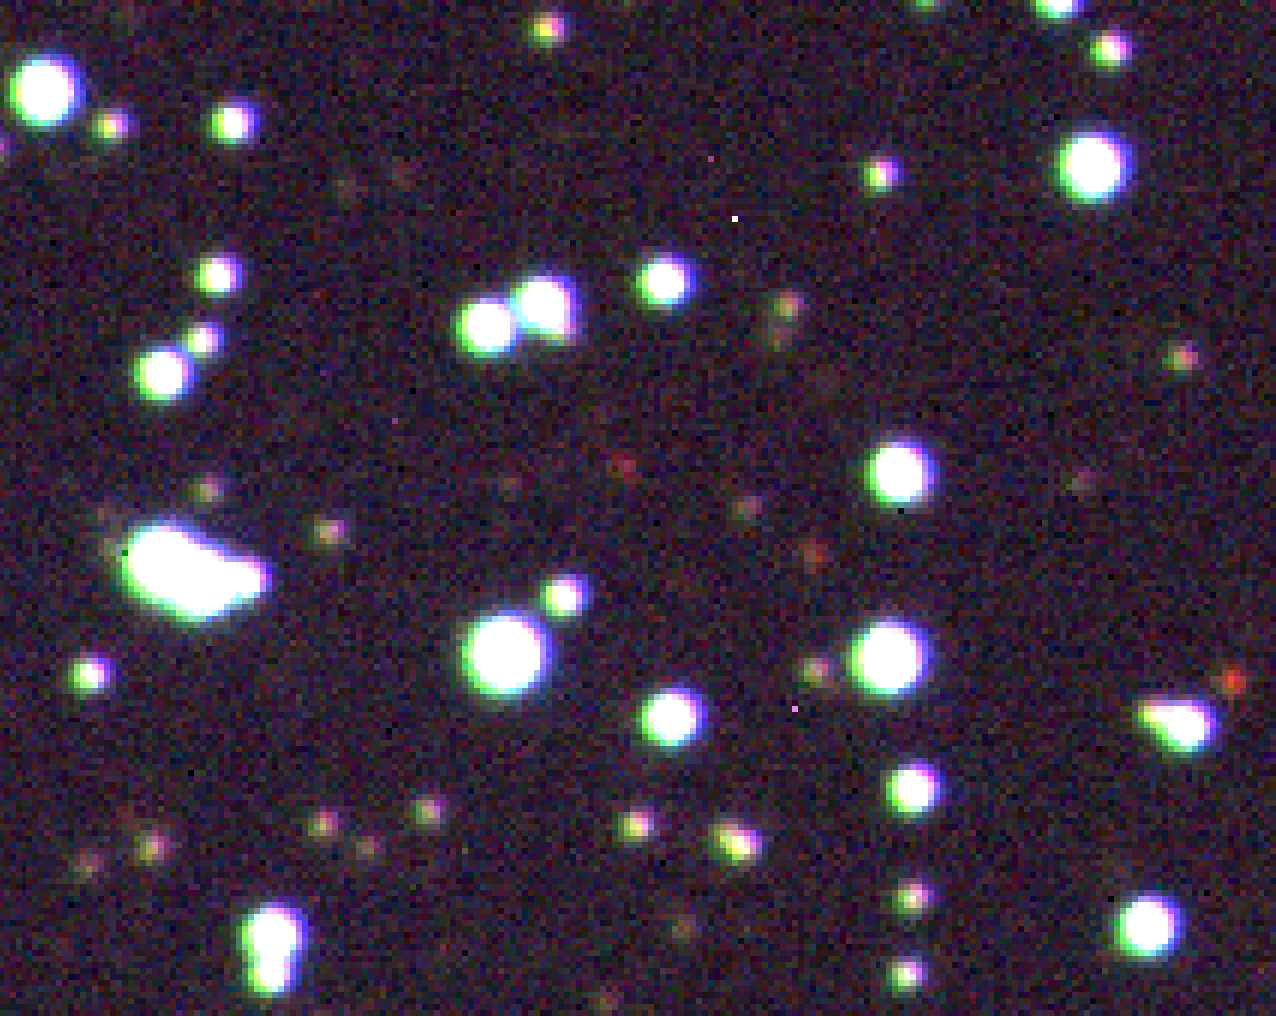
\includegraphics[width=0.5\textwidth]{inventing-color/rgb-bad}
	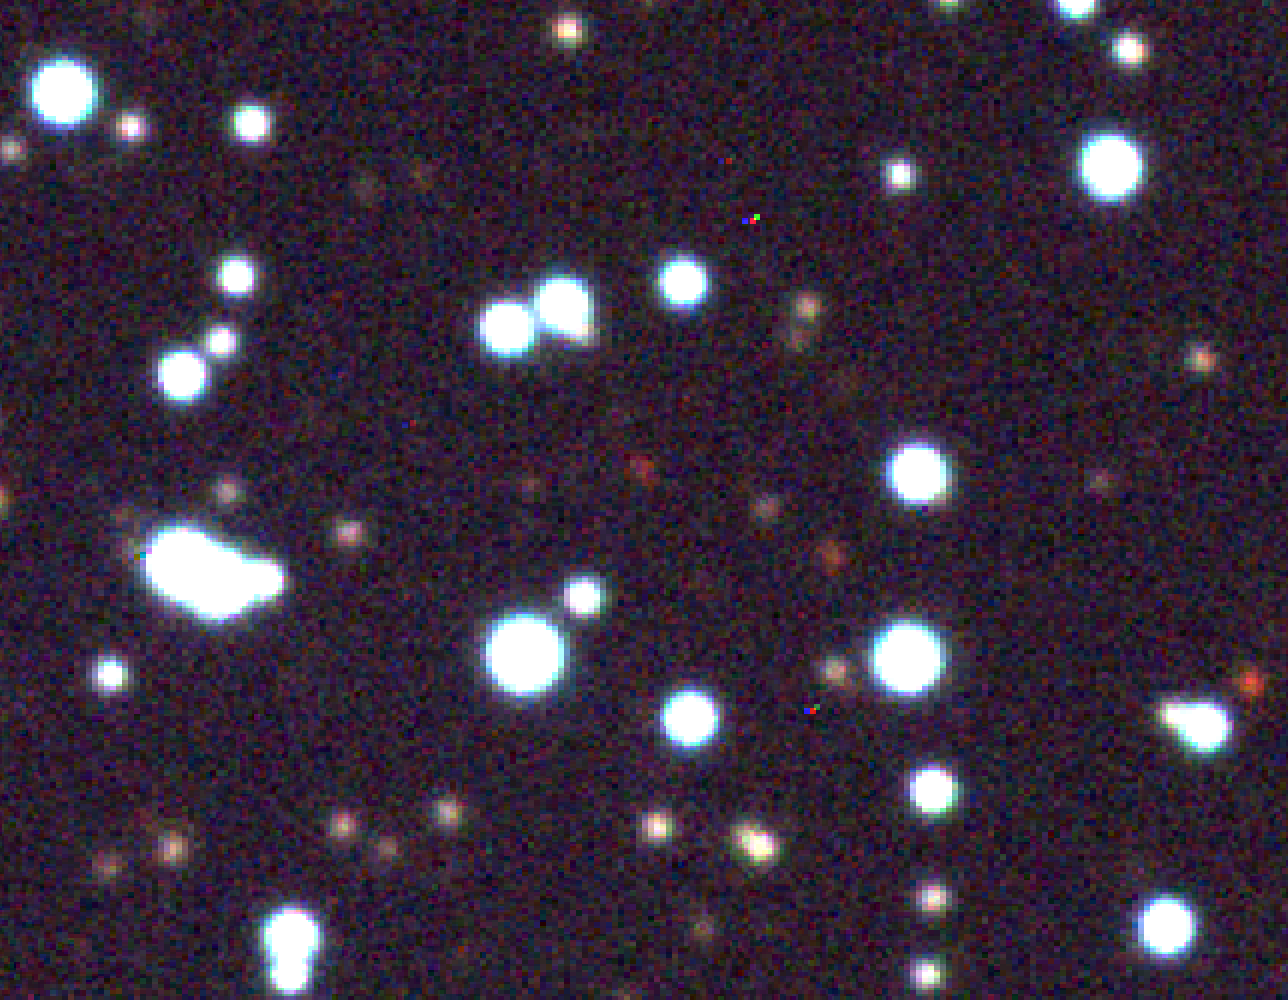
\includegraphics[width=0.5\textwidth]{inventing-color/rgb-good}
	\caption{Zoom-in on a color image, showing poor (left) and good (right) image alignment across filters. Note how objects are shifted between different color channels in the poorly aligned image.}\label{ic:fig:rgb-bad}
\end{figure}

\section{Report checklist and grading}

Each item below is worth 10 points. See Appendix\ \ref{cha:lab-report-format} for guidance on writing the report and formatting tables and graphs.

\begin{enumerate}

	\item List of team role assignments and agreements about group communication (Step \ref{ic:step:team-comm}).

	\item Pattern of how shape of spectrum changes with temperature, your peak wavelength, and how to use spectrum to predict color (Steps \ref{ic:step:load-sim}--\ref{ic:step:qual-color}).
	
	\item Observations of how spectrum and filter magnitudes change with temperature (Step \ref{ic:step:see-thermal}).
	
	\item Table and graph of color index versus temperature (Step \ref{ic:step:tempcolor}).
	
	\item Procedure, calculations, and determination of solar temperature and uncertainty.
	
	\item Comparison with percent difference, $t'$ statistic, and discussion (Steps \ref{ic:step:proc-color}--\ref{ic:step:solar-compare}).
	
	\item Your beautiful color image (Step \ref{ic:step:color-image}).
	
	\item Discuss the findings and reflect deeply on the quality and importance of the findings. This can
	be both in the frame of a scientist conducting the experiment (“What did the experiment tell us
	about the world?”) and in the frame of a student (“What skills or mindsets did I learn?”).
	
%	\item A 100–200 word reflection on group dynamics and feedback on the lab manual. Address the
%	following topics: who did what in the lab, how did you work together, what successes and
%	challenges in group functioning did you have, and what would you keep and change about the
%	lab write-up?
	
	\item Write a paragraph (100--200 words) reporting back from each of the four roles: facilitator, scribe, technician,
	skeptic. Where did you see each function happening during this lab, and where did you see gaps? Which did you do, and how did that go? what successes and	challenges in group functioning did you have, and what would you keep and change about the
	lab write-up?
\end{enumerate}
